% ! TEX root = ../semdis.tex

\chapter{Aplicație: Coerența semantică \\ în poezia modernă}

Prezentăm acum aplicația din articolul \cite{herbelot}, asupra coerenței
semantice în poezia modernă și contemporană, aplicație care vine în
continuarea considerațiilor teoretice generale din capitolul anterior.

\section{Teoria lucrării}

Pentru a susține teza că poeziile folosesc o structură similară a limbii
cu limbajul comun atunci cînd produc construcții cu sens, ar trebui să
arătăm că limbajul poetic este caracterizat de o \emph{coerență a subiectelor}
(eng.\ \emph{topic coherence}). Ideea de bază a acestei cercetări este să
folosească metode distribuționale pentru a arăta că, de exemplu, mulțimea de
subiecte $ \{ $ scaun, masă, birou, echipă $ \} $ are o coerența mai mare
decît $ \{ $ scaun, rece, elefant, nor $ \} $.

Poeziile studiate sînt scrise în perioada 1881-2008 și variază, ca stil,
de la unele considerate dificile, la altele, \qq{transparente}.

Se definește \emph{coerența unei mulțimi de cuvinte} (cf.\ \cite{newman})
$ \{ w_1, w_2, \dots, w_n \} $ ca fiind media similarităților lor în perechi
(două cîte două):
\[
  \overline{S}(w) = \overline{\{ \dr{Sim}(w_i, w_j) \mid 1 \leq i < j \leq n \} },
\]
unde bara superioară notează media. Similaritatea se definește cu ajutorul
cosinusului:
\[
  \dr{Sim}(A, B) = \dfrac{\sum_{i=1}^n A_i \cdot B_i}{\sqrt{\sum_{i=1}^n A_i^2} %
    \cdot \sqrt{\sum_{i=1}^n B_i^2}},
\]
unde $ n = 2000 $ (vezi mai jos).

Corpusul folosit face parte din British National Corpus, care a fost lematizat
și s-au asociat etichete folosind sistemul \href{http://ucrel.lancs.ac.uk/claws/}{CLAWS},
pe care nu îl detaliem, pentru că modul său de funcționare și implementare
este irelevant pentru restul prezentării.

În plus, se ignoră punctuația, iar cuvintele-cheie fac parte din categoriile:
substantive, verbe, adjective și adverbe. Fiecare poezie studiată se convertește
în secvențe de cîte 11 cuvinte, iar contextul asociat unui cuvînt-cheie înseamnă
cele 5 cuvinte care îl precedă și cele 5 care îl urmează.

Co-ocurențele se calculează folosind formulele:
\begin{align*}
  \dr{freq}(c_i) &= \displaystyle\sum_t \dr{freq}(c_i, t) \\
  \dr{freq}(t) &= \sum_{c_i} \dr{freq}(c_i, t) \\
  \dr{freq}(\text{total}) &= \sum_{c_i, t} \dr{freq}(c_i, t),
\end{align*}
unde:
\begin{itemize}
\item $ \dr{freq}(c_i, t) $ este frecvența cuvîntului $ c_i $, care este
  context, făcînd parte din contextul asociat cuvîntului-țintă $ t $;
\item $ \dr{freq}(\dr{total}) $ este numărul total de cuvinte;
\item $ \dr{freq}(t) $ este frecvența cuvîntului-țintă $ t $;
\item $ \dr{freq}(c_i) $ este frecvența cuvîntului de context $ c_i $.
\end{itemize}

Apoi, se calculează ponderea fiecărui termen de context cu formula:
\[
  v_i(t) = \dfrac{p(c_i \mid t)}{p(c_i)} = \dfrac{\dr{freq}(c_i, t) \cdot %
    \dr{freq}(\text{total})}{\dr{freq}(t) \cdot \dr{freq}(c_i)}.
\]

Se aleg primele 2000 cele mai frecvente cuvinte din corpus ca bază
a spațiului semantic. Numărul ales s-a dovedit a fi relevant și în
alte experimente.

%%%%%%%%%%%%%%%%%%%%%%%%%%%%%%%%%%%%%%%%%%%%%%%%%%%%%%%%%%%%%%%%%%%%%%

\section{Experimentul}

Au fost alexe 8 poezii scrise în limba engleză modernă, de diverse grade de
dificultate, adică cerînd diferite nivele de profunzime a analizei pentru
a identifica sensul. Se mai folosesc și două texte de control: un articol
din Wikipedia și un text generat aleatoriu, pentru a servi drept margine
superioară, respectiv inferioară în ce privește structura frazeologică,
semantică și coerență. În fine, s-au atribuit scoruri de dificultate de către
autor și doi referenți independenți, unde scorul de 1 înseamnă foarte ușor
de înțeles, iar scorul de 5 înseamnă foarte greu de înțeles.

Textele alese sînt prezentate în tabelul din figura \ref{fig:tab-poezii}.
Mai multe detalii privitoare la autori și texte considerăm că sînt irelevante
pentru scopul lucrării prezente.

\begin{figure}[!htb]
  \centering
  \begin{tabular}{l|l|l}
    Autor & Titlu & An \\
    \hline
    Brooke & Day That I Loved & 1911 \\
    Coolidge & Argument Over, Amounting & 1990 \\
    Duffy & Valentine & 1993 \\
    Ginsberg & Five A.\ M.\ & 1996 \\
    MacCormack & At Issue III & 2001 \\
    Slater & Ithaca, Winter & 2008 \\
    Stein & If I Told Him, \newline A Completed Portrait of Picasso & 1924 \\
    Wilde & In the Gold Room & 1881 \\
    Wikipedia & The Language Poets & ? \\
    Random & Psychologist. String & N/A
  \end{tabular}
  \caption{Poeziile alese în experimentul pentru coerență din \cite{herbelot}}
  \label{fig:tab-poezii}
\end{figure}

Scorurile de dificultate au fost:

\begin{figure}[!htb]
  \centering
  \begin{tabular}{l|l|l|l|l}
    Textul & Autorul & Referent 1 & Referent 2 & Media \\
    \hline
    Random & 5 & 5 & 5 & 5 \\
    MacCormack & 5 & 5 & 5 & 5 \\
    Coolidge & 4 & 5 & 5 & 4.67 \\
    Ginsberg & 5 & 4 & 3 & 4 \\
    Stein & 5 & 3 & 3 & 3.67 \\
    Slater & 2 & 3 & 4 & 3 \\
    Brooke & 2 & 4 & 3 & 3 \\
    Wilde & 1 & 1 & 2 & 1.33 \\
    Duffy & 1 & 1 & 2 & 1.33 \\
    Wikipedia & 1 & 1 & 1 
  \end{tabular}
  \caption{Scorurile de dificultate atribuite textelor alese în \cite{herbelot}}
\end{figure}

Poeziile au fost etichetate POS\footnote{\href{https://en.wikipedia.org/wiki/Part-of-speech\_tagging}{parts-of-speech}}
automat, dar etichetarea a fost apoi verificată manual.

S-a calculat coerența pentru poeziile care au o structură frazeologică destul
de clară (Brooke, Duffy, Slater, Stein, Wilde, random, Wikipedia), iar pentru
celelalte, s-a efectuat o împărțire în diviziuni cu același numă de cuvinte.
De asemenea, în conformitate cu ipotezele de lucru, s-au luat în considerare doar
părțile relevante de propoziție care au apărut de cel puțin 50 de ori. În total,
s-a folosit aproximativ 72\% din conținutul textual, iar lungimea medie a
frazelor a fost de 4 cuvinte relevante.

%%%%%%%%%%%%%%%%%%%%%%%%%%%%%%%%%%%%%%%%%%%%%%%%%%%%%%%%%%%%%%%%%%%%%%

\section{Rezultate și concluzii}

Cel mai clar se pot vedea rezultatele pe graficul din figura
\ref{fig:coerenta1}.

\begin{figure}[!htb]
  \centering
  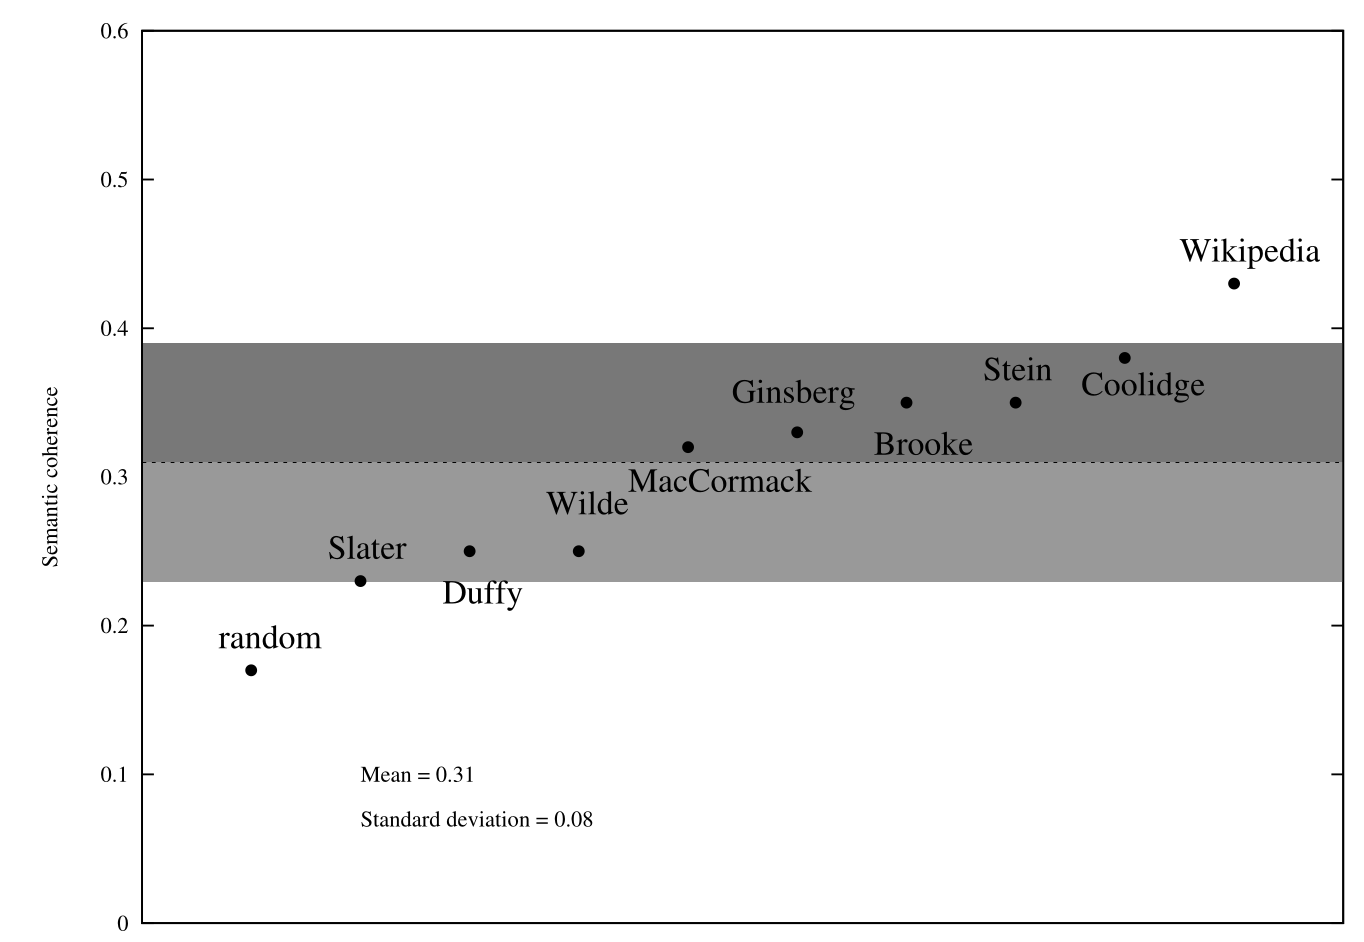
\includegraphics[scale=0.3]{img/coherence1.png}
  \caption{Coerența subiectelor din experimentul prezentat în \cite{herbelot}}
  \label{fig:coerenta1}
\end{figure}


Se poate vedea aici că textele poetice analizate se situează aproape la mijloc
din punctul de vedere al coerenței între textul aleatoriu și cel de pe
Wikipedia. Pentru a elimina anumite îndoieli, autoarea au mai adăugat cîteva
texte aleatorii și cîteva de pe Wikipedia, graficul accentuîndu-se și mai bine,
ca în figura \ref{fig:coerenta2}.

\begin{figure}[!htb]
  \centering
  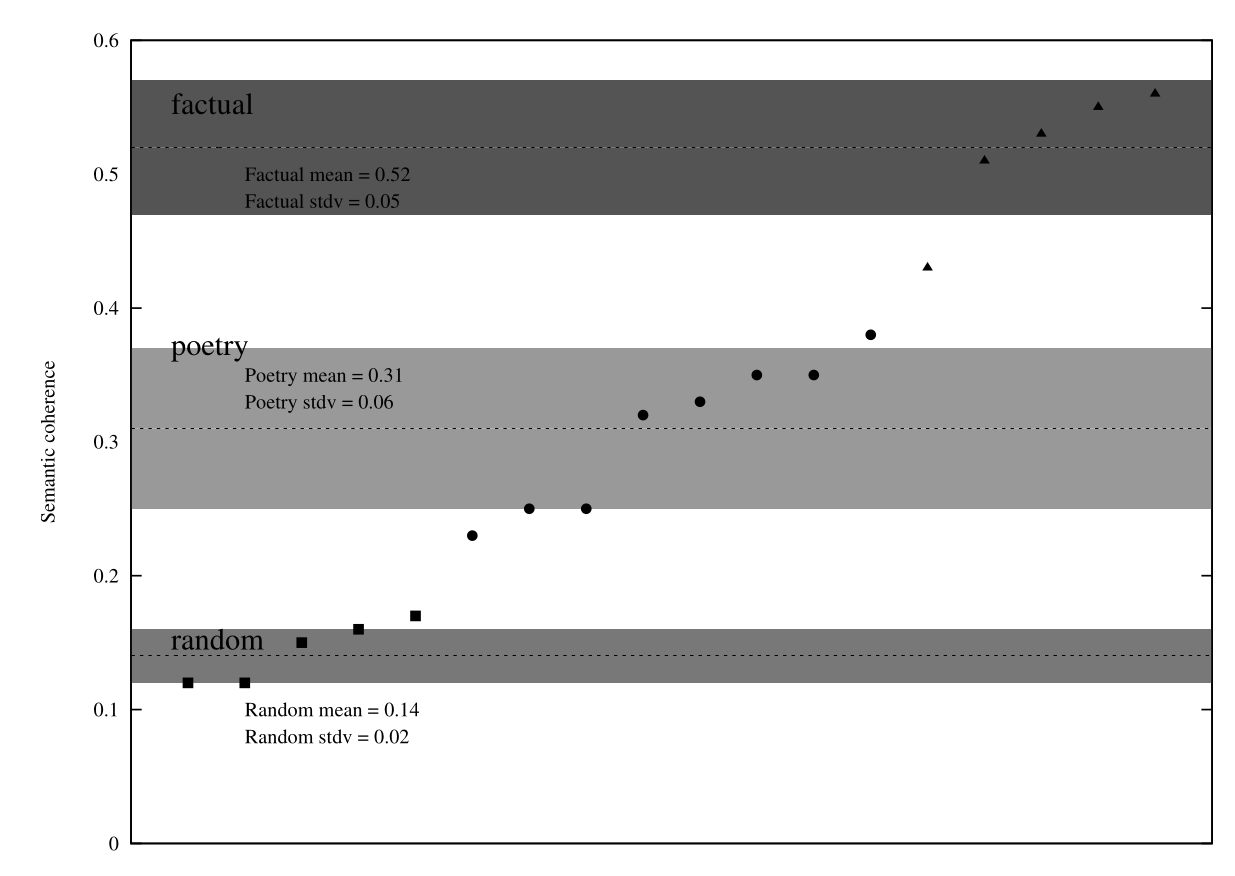
\includegraphics[scale=0.35]{img/coherence2.png}
  \caption{Coerența subiectelor din experimentul prezentat în \cite{herbelot},
  cu texte de control adăugate suplimentar}
  \label{fig:coerenta2}
\end{figure}

Ideile de bază care se desprind din aceste rezultate sînt că, pe de o parte,
poezia produsă de oameni se poate distinge destul de ușor de texte aleatorii,
dar și că există o diferență semnificativă între textele științifice ori
factuale (precum articolele de pe Wikipedia) și cele poetice. Totodată,
coerența poeziilor este mai scăzută decît cea a textelor factuale, rezultat
care se explică prin creativitatea autorului.

Mai trebuie remarcat și faptul că nu există nicio corelație între dificultatea
textului, așa cum a fost ea percepută de oameni, și coerența care rezultă
din calcule. De exemplu, poeziile lui Duffy și Wilde, considerate "ușoare",
nu au un factor de coerență mare, lucru care este pus pe seama creativității
autorilor. Rezultă, deci, că semantica nu lipsește cu precădere din textele
complicate, așa cum afirmă unii critici.

Concluziile pe care le putem desprinde, împreună cu autoarea \cite{herbelot},
sînt de felul următor. Folosind punctul de vedere distribuțional asupra
sensului, este, într-adevăr, posibil să se pună în evidența relația între
limbajul comun și cel \qq{neobișnuit}, al poeziei. În același timp, tot
modelul distribuțional arată clar distincția între texte umane și cele
produse aleatoriu, indiferent de transparența sau dificultatea textului.
Acest lucru se poate vedea foarte bine pe graficele care arată coerența,
indicate mai sus.


%%% Local Variables:
%%% mode: latex
%%% TeX-master: "../semdis"
%%% End:
